\begin{figure*}

\begin{subfigure}{\textwidth}
\begin{minipage}[b]{0.7365\textwidth}
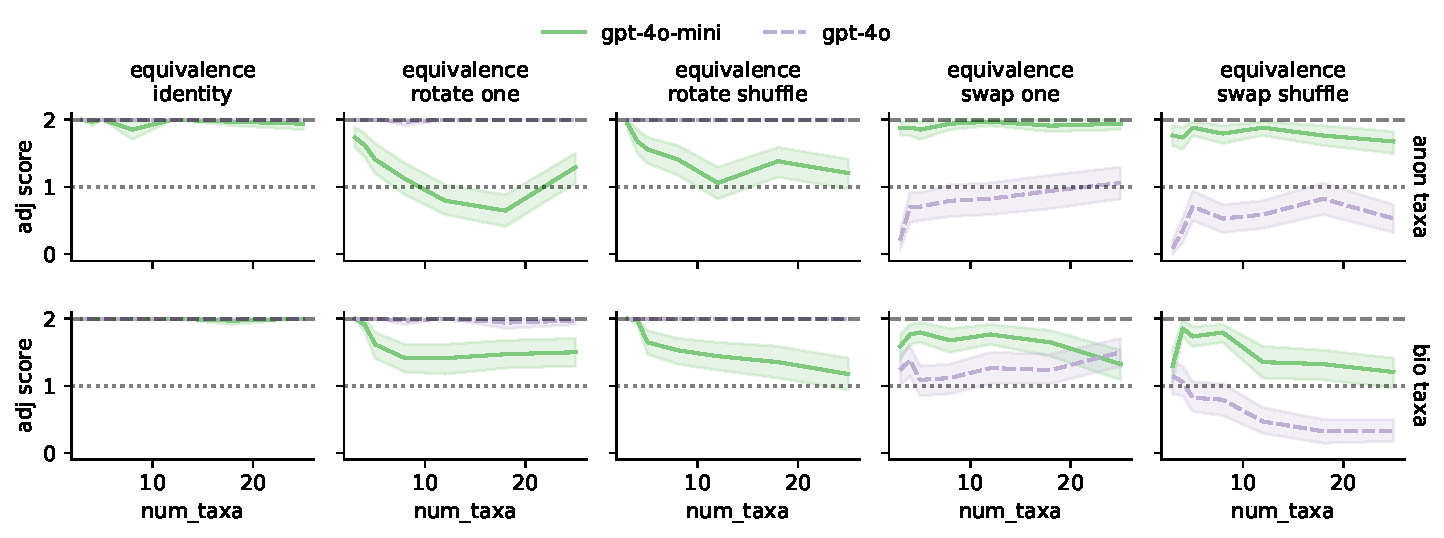
\includegraphics[width=\textwidth, trim={0cm 0cm 1cm 1cm}, clip]{binder/binder-2024-11-07-scientific.ipynb/binder/teeplots/2024-11-07-scientific/col=q+hue=model+is_equivalence=True+kind=line+palette=accent+repr_=json+row=tree-source+style=model+viz=relplot+x=num-taxa+y=adj-score+ext=.pdf}
\end{minipage}%
\begin{minipage}[b]{0.01\textwidth}
\end{minipage}
\begin{minipage}[b]{0.2535\textwidth}
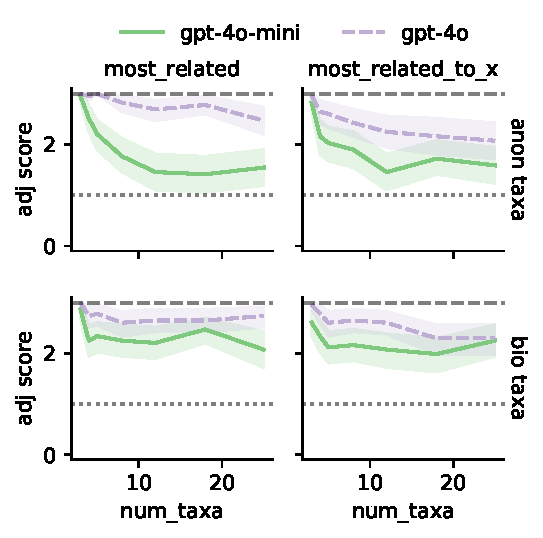
\includegraphics[width=\textwidth, trim={0.65cm 0cm 0cm 0cm}, clip]{binder/binder-2024-11-07-scientific.ipynb/binder/teeplots/2024-11-07-scientific/col=q+hue=model+is_equivalence=False+kind=line+palette=accent+repr_=json+row=tree-source+style=model+viz=relplot+x=num-taxa+y=adj-score+ext=.pdf}
\end{minipage}
\caption{JSON representation}
\label{fig:models:json}
\end{subfigure}

\begin{subfigure}{\textwidth}
\begin{minipage}[b]{0.7365\textwidth}
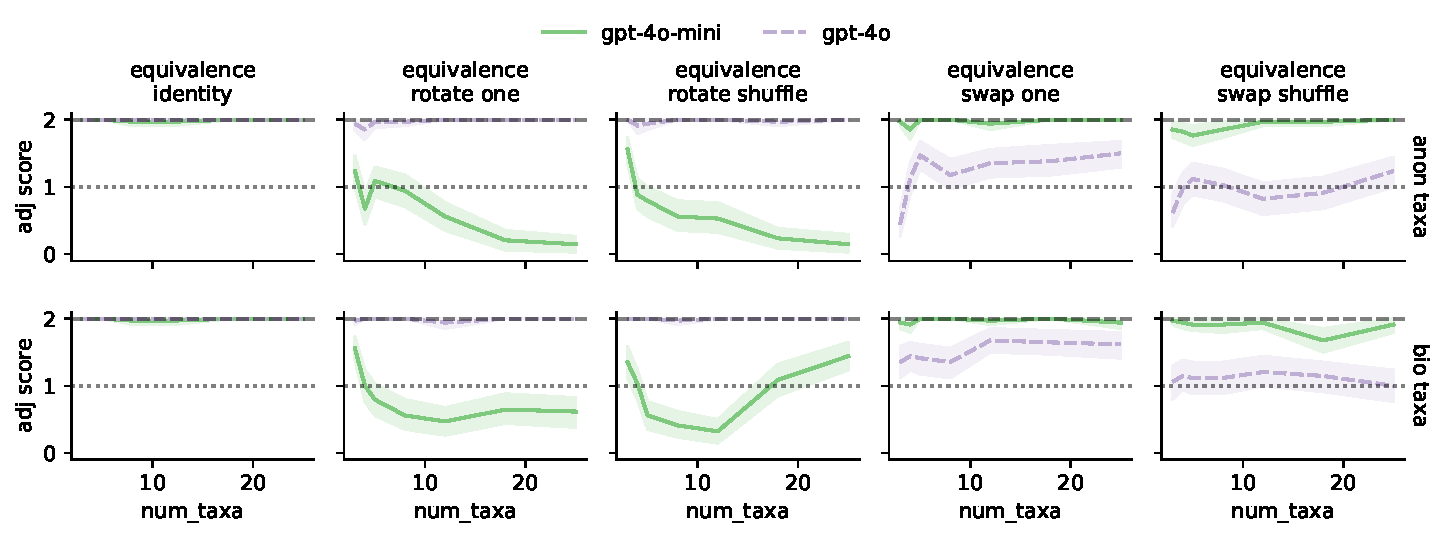
\includegraphics[width=\textwidth, trim={0cm 0cm 1cm 1cm}, clip]{binder/binder-2024-11-07-scientific.ipynb/binder/teeplots/2024-11-07-scientific/col=q+hue=model+is_equivalence=True+kind=line+palette=accent+repr_=newick+row=tree-source+style=model+viz=relplot+x=num-taxa+y=adj-score+ext=.pdf}
\end{minipage}%
\begin{minipage}[b]{0.01\textwidth}
\end{minipage}
\begin{minipage}[b]{0.2535\textwidth}
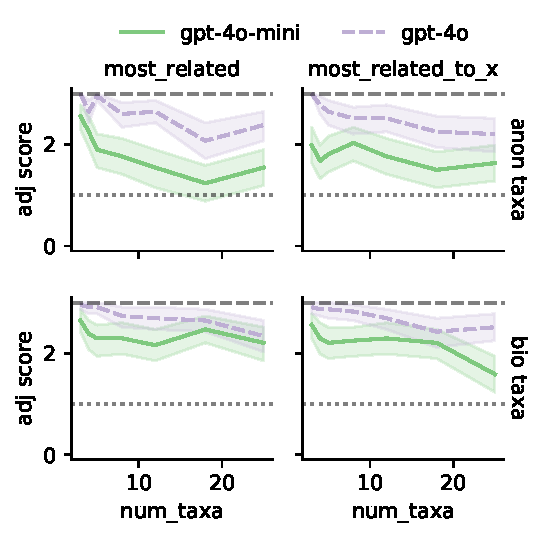
\includegraphics[width=\textwidth, trim={0.65cm 0cm 0cm 0cm}, clip]{binder/binder-2024-11-07-scientific.ipynb/binder/teeplots/2024-11-07-scientific/col=q+hue=model+is_equivalence=False+kind=line+palette=accent+repr_=newick+row=tree-source+style=model+viz=relplot+x=num-taxa+y=adj-score+ext=.pdf}
\end{minipage}
\caption{Newick representation}
\label{fig:models:newick}
\end{subfigure}

\begin{subfigure}{\textwidth}
\begin{minipage}[b]{0.7365\textwidth}
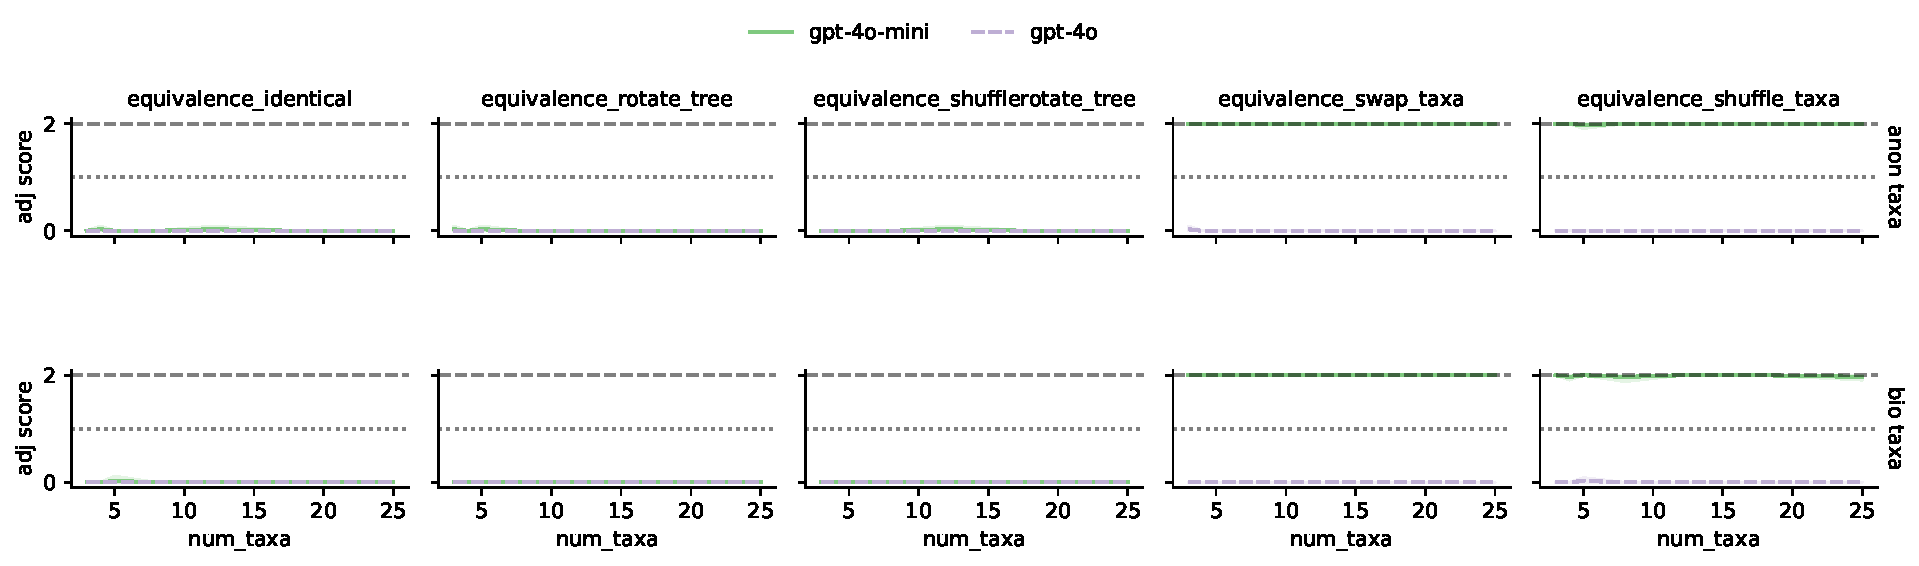
\includegraphics[width=\textwidth, trim={0cm 0cm 1cm 1cm}, clip]{binder/binder-2024-11-07-scientific.ipynb/binder/teeplots/2024-11-07-scientific/col=q+hue=model+is_equivalence=True+kind=line+palette=accent+repr_=none+row=tree-source+style=model+viz=relplot+x=num-taxa+y=adj-score+ext=.pdf}
\end{minipage}%
\begin{minipage}[b]{0.01\textwidth}
\end{minipage}
\begin{minipage}[b]{0.2535\textwidth}
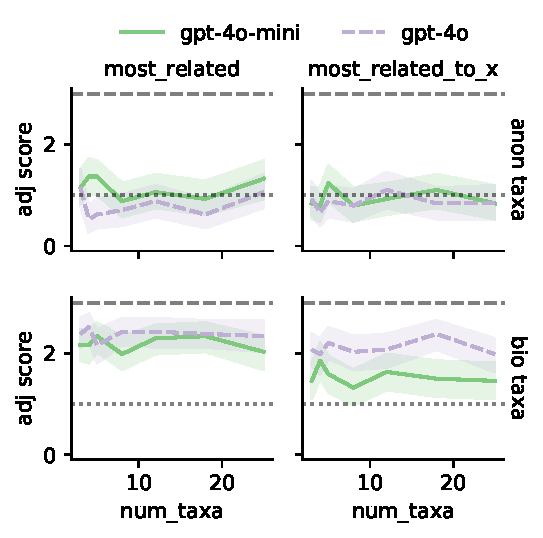
\includegraphics[width=\textwidth, trim={0.65cm 0cm 0cm 0cm}, clip]{binder/binder-2024-11-07-scientific.ipynb/binder/teeplots/2024-11-07-scientific/col=q+hue=model+is_equivalence=False+kind=line+palette=accent+repr_=none+row=tree-source+style=model+viz=relplot+x=num-taxa+y=adj-score+ext=.pdf}
\end{minipage}
\caption{Blank representation (no tree shown)}
\label{fig:models:blank}
\end{subfigure}

\caption{
\textbf{Model comparison.}
Shaded bands denote bootstrapped 95\% CI, $n=100$.
}
\label{fig:models}

\end{figure*}
